\documentclass[11pt]{report}
\usepackage[a4paper]{geometry}
\usepackage{outline}
\usepackage{pmgraph}
\usepackage[normalem]{ulem}
\usepackage{graphicx}
\usepackage{booktabs}
\usepackage{amsmath}
\usepackage{amsthm}
\usepackage{eucal}
\usepackage{amssymb}
\usepackage{mathrsfs}
\begin{document}
%-------------------------------------------------------------------
%-------------------------------------------------------------------
\part{Google's PageRank and Beyond - Langville and Meyer}
\chapter{Ranking Web pages by popularity}
\section{Two thesis}
\textbf{Hyperlink} structure forms a massive directed graph - nodes in the graph represent web pages and links represent the hyperlinks, \textbf{inlinks} point into nodes, \textbf{outlinks} point out from nodes
\subsection{PageRank}
Page with more recommendations must be more important than a page with a few inlinks, status of recommender also important. \textit{PageRank's thesis is that a webpage is important if it is pointed to by other important pages.}
\subsection{HITS}
\begin{itemize}
\item Uses both inlinks and outlinks to create two popularity scores for each page
\item Hub if contains many outlinks
\item Authority if it has many inlinks
\item \textit{A page is a good hub(and therefore deserves a high hub score) if it points to good authorities, and a page is a good authority if its pointed to by good hubs.}
\end{itemize}
\section{Query-Independence}
\begin{itemize}
\item Query-independent if the popularity score for each page is determined off-line, remains constant until next query
\item At query time, no time is spent computing popularity scores for relevant pages
\item PageRank - query-independent
\item HITS - originally query-dependent
\end{itemize}
%---------------------------------------------------------------------
\chapter{The Mathematics of Google's PageRank}
PageRank importance scores are actually the stationary values of an enormous Markov chain
\section{The Original Summation Formula for PageRank}
\begin{itemize}
\item \begin{equation}
r(P_i) = \displaystyle \sum_{P_j\in B_{P_i }} \frac{r(P_j)}{|P_j|} 
\end{equation} where $B_{P_i }$ is the set of pages pointing into $P_i$, and $\vert P_j \vert $ is the number of outlinks from the page 
\item Outlink ranks are unknown 
\item Use iterative procedure
\begin{itemize}
\item Assume all pages have equal PageRank $\frac{1}{n}$ 
\begin{equation}
r_{(k+1)}P_i = \displaystyle \sum_{P_j\in B_{P_i }}\frac{r_k(P_j)}{|P_j|}
\end{equation}
\item Initiated with \(r_0(P_i) = \frac{1}{n}\)
\end{itemize}
\end{itemize}
\section{Matrix representation}
\begin{itemize}
\item Replace sum, at each iteration compute a PageRank vector which holds PageRank values for all pages in the index
\item Introduce a \textit{n} x \textit{n} matrix \textbf{H} and a 1 x \textit{n} row vector $\boldsymbol{\pi}^T$
\item \textbf{H} row normalized hyperlink matrix with $\boldsymbol{H_{ij}} = \begin{cases} \frac{1}{P_j} &  \textnormal{if there is a link from node i to j}  \\ 0 & otherwise\end{cases}$ 
\item \textbf{H} non-zero elements are probabilities
\item Write the summation formula as \begin{equation}
\boldsymbol{\pi}^{(k+1)T} = \boldsymbol{\pi}^{(k)T}\textbf{H}
\end{equation}
\item Matrix reveals some immediate observations:
\begin{enumerate}
\item Each iteration involves one vector-matrix multiplication
\item Sparse matrix, most webpages only link to average 10 other pages - require minimal storage, requires \textit{O(nnz}\textbf{H}), linear
\item Classical power method applied to \textbf{H}
\item \textbf{H} looks like a stochastic transition probabilty matrix for a Markov chain
\end{enumerate}
\end{itemize}
\section{Problems with the Iterative Process}
\begin{itemize}
\item Rank sinks, pages that accumulate PageRank with each iteration - dangling nodes and cycles
\item Prefer PageRank vector to be positive
\end{itemize}
\section{Markov theory}
\begin{itemize}
\item Power method applied to a Markov chain with transition probabilty matrix \textbf{H}
\item Know for any starting vector, the power method on a matrix converges to a stationary vector as long as the matrix is stochastic, irreducible and aperiodic (aperiodicity and irreducibility implies primitvity)
\end{itemize}
\section{Early Adjustments}
\begin{itemize}
\item Grand application of Markov chains
\item Random surfer idea
\item \textbf{Stochasticity adjustment} - where rows of 0’s are changed to rows of 1/n. In terms of the random surfer, this means that if it enters a dangling node it can jump to another page at random 
\item \begin{equation}
\textbf{S} = \textbf{H} + \textbf{a}(\frac{1}{n}\cdot 1^{T}
\end{equation}
\item \textbf{a} is the dangling node vector, \textbf{S} is the stochastic matrix
\item Guarantees that S is stochastic, and is the transition probabilty matrix for a Markov chain - but not convergence
\item \textbf{Primitivity adjustment} - random surfer follows \textbf{S} with probability \(\alpha\), but can jump to a random page with probability \(1-\alpha\), forming the Google Matrix \textbf{G}
\item \begin{equation}
\textbf{G} = \alpha\textbf{S} + (1-\alpha)\cdot\frac{1}{n}\cdot 1^{T}
\end{equation}
\item Teleporting is random, equally likely to jump to any page
\item Several consequences of the primitivity adjustment
\begin{enumerate}
\item \textbf{G} is stochastic, combination of two stochastic matrices
\item \textbf{G} is irreducible
\item \textbf{G} is aperiodic
\item \textbf{G} is primitive, because \(\textbf{G}^k>0\) for some k, implies that a unique positive \(\boldsymbol{\pi}^T\) exists, and the power method applied to \textbf{G} is guaranteed to converge to this vector
\item \textbf{G} is dense, bad thing computationally, can be written in terms of the sparse \textbf{H}
\begin{equation}
\begin{split}
\textbf{G} &= \alpha\textbf{S} + (1-\alpha)\cdot\frac{1}{n}\cdot 1^{T}\\
&= \alpha(\textbf{H} +\frac{1}{n}\textbf{a}\cdot1^{T}) + (1-\alpha)\cdot\frac{1}{n}\cdot1^T \\
&= \alpha\textbf{H} + (\alpha\textbf{a}+(1-\alpha))\frac{1}{n}\cdot1^T
\end{split}
\end{equation}
\item \textbf{G} is artificial, modified twice in order to produce desirable convergence properties
\end{enumerate}
\item Google's adjusted PageRank method is the power method applied to \textbf{G} \begin{equation}
\boldsymbol{\pi}^{(k+1)T} = \boldsymbol{\pi}^{(k)T}\textbf{G}
\end{equation}
\end{itemize}
\section{Computation of PageRank vector}
\begin{itemize}
\item Problem can be stated in two ways
\begin{enumerate}
\item Solve the following eigenvector problem for $\pi^T$ \begin{eqnarray}
\boldsymbol{\pi}^T = \boldsymbol{\pi}^T\textbf{G}\\
\boldsymbol{\pi}^T\textbf{e}=1
\end{eqnarray}
\item Solve the following linear homogeneous system for $\pi^T$
\begin{eqnarray}
\boldsymbol{\pi}^T(\textbf{I}-\textbf{G})=\textbf{0}^T\\
\boldsymbol{\pi}^T\textbf{e}=1
\end{eqnarray}
\end{enumerate}
\item In 1. goal is to find a normalized dominant left-hand eigenvector of \textbf{G} corresponding to the dominant eigenvalue $\lambda_1 = 1$
\item In 2. want to find normalized left-hand null vector of \textbf{I} - \textbf{G}
\item Power method
\begin{itemize}
\item Slow
\item Simple
\item Vector-matrix multiplication can be done on sparse \textbf{H}, \textbf{S} and \textbf{H} are never formed or stored, only rank one components \textbf{a} and \textbf{e} are needed
\item Matrix-free
\item Storage friendly, sparse matrix, dangling node vector and current iterate need to be stored, n real numbers - GMRES(10) require 10n
\item 50-100 iterations needed - 2/3 degrees of accuracy
\end{itemize}
\end{itemize}
%-----------------------------------------------------------------
\chapter{Parameters in the PageRank Model}
\section {The $\alpha$ factor}
\begin{itemize}
\item $\alpha$ controls the priority given to the Web's natural hyperlink structure
\item 0.85 is workable compromise between efficiency and effectiveness
\item Affects sensitivity of resulting PageRank vector
\item As $\alpha\rightarrow 1$, artificiality reduces, but computation time increases
\item As $\alpha\rightarrow 1$ PageRankings become more volatile
\end{itemize}
\section{The Hyperlink matrix \textbf{H}}
\begin{itemize}
\item Random surfer may not be accurate at all - equality not best for webpages
\item Replace with \textbf{intelligent surfer}
\item May be more likely to jump to a more content-filled pages, so these pages should be given more probabilistic weight
\item Practical way to do this - use access logs to find actual surfer tendencies, and then adjust probabilities in \textbf{H} accordingly
\item Other methods to fill elements in \textbf{H} - REFERENCES \textbf{Baeza-Yates,Davis} \textit{Web page ranking using link attributes}, \textbf{Bharat, Henzinger} \textit{Improved algorithms for topic distillation}, \textbf{Bharat, Maghoul, Stata}, \textit{The term vector database}, \textbf{Richardson, Domingos}, \textit{The intelligent surfer;Probablistic combination of link and content information in PageRank}, \textbf{Tomlin}, \textit{A new paradigm for ranking pages on the WWW}
\item These methods use heuristic (hands-on) rules to create the nonzero elements of \textbf{H} by combining location of outlinks, length of anchor text, and content similarity
\end{itemize}
\section{The Teleportation Matrix E}
\begin{itemize}
\item Rather than use $\frac{1}{n}1^T$, used $\textbf{ev}^T$ where $\textbf{v}^T >0$ is the personalization vector
\item Using personalization vector, means that the probabilties are no longer uniformly distributed
\item Retains the advantageous properties of power method
\item When $\textbf{G} = \alpha\textbf{S}+(1-\alpha)\textbf{ev}^T$ \begin{equation}
\begin{split}
\boldsymbol{\pi}^{(k+1)T} &=\boldsymbol{\pi}^{(k)T}\textbf{G}\\
&=\alpha\boldsymbol{\pi}^{(k)T}\textbf{S} + (1-\alpha)\boldsymbol{\pi}^{(k)T}\textbf{ev}^T\\
&=\alpha\boldsymbol{\pi}^{(k)T}\textbf{H}+(\alpha\boldsymbol{\pi}^{(k)T}\textbf{a}+1-\alpha)\textbf{v}^T
\end{split}
\end{equation}
\item Only thing that changes is the PageRank vector itself, different personalizations produce different PageRankings REFERENCE: \textbf{Thorson}, \textit{Modeling the web and the computation of PageRank}
\item $\boldsymbol{\pi}^T(\textbf{v}^T)$ is a function of $\textbf{v}^T$
\item Original says nothing about me and my preferences
\item In practice is computationally impossible
\item Pseudo-personalized PageRanking systems, REFERENCE: \textbf{Haveliwala}, \textit{Efficient computation of PageRank}
\item Haveliwala - topic sensitive Page Rank
\begin{itemize}
\item Finite number of PageRank vectors each biased towards a particular topic
\item 16 top-level topics - Arts, Business etc.
\item Biased PageRank vectors calculated ahead of time
\item Topic-sensitive, query-dependant PageRank vector as a convex combination of PageRank vectors
\item Uses a Bayesian classifier to compute the $\beta_i$'s for the experiments
\end{itemize}
\item Personalization vector could be used to control spamming by link farms
\end{itemize}
%-----------------------------------------------------------------
\chapter{The HITS Method for Ranking Webpages}
\section{The HITS Algorithm}
\begin{itemize}
\item Hypertext Induced Topic Search - Jon Kleinberg in 1998
\item Like PageRank, uses web hyperlink to create popularity scores associated with webpages
\item HITS produces two popularity scores, query dependant
\item Thinks of web pages as authorities and hubs
\item An authority is a page with many inlinks, a hub is a page with many outlinks
\item Good authorities are pointed to by good hubs, and good hubs point to good authorities
\item Every page is some measure of an authority and some measure of a hub
\item Mathematics
\begin{itemize}
\item Every page has both an authority score $x_i$ and a hub score $y_i$
\item Let E be the set of all directed edges in the web graph and let $e_{ij}$ represent the directed edge from node \textit{i} to node \textit{j}
\item Each page is assigned initial authority score $x_i^{(0)}$ and initial hub score $y_i^{(0)}$, redefines by computing \begin{equation}
x_i^{(k)} = \displaystyle \sum_{j:e_{ij}\in E} y_j^{(k-1)} \quad\mathrm{and}\quad y_i^{(k)} = \displaystyle \sum_{j:e_{ij}\in E} x_j^{(k)}  \quad\mathrm{for}\quad k=1,2,3\ldots
\end{equation}
\item These can be written in matrix with the use of adjacency matrix \textbf{L} of the directed graph \begin{equation}
\textbf{L}_ij = \begin{cases} 1, & \textnormal{if there exists an edge from node \textit{i} to node \textit{j}}\\ 0 & \textnormal{otherwise}
\end{cases}
\end{equation}
\item In matrix notation, the equations become \begin{equation}
\textbf{x}^{(k)} = \textbf{L}^T\textbf{y}^{(k-1)}\quad\mathrm{and}\quad \textbf{y}^{(k)}=\textbf{Lx}^{(k)}
\end{equation} where \(\textbf{x}^{(k)}\) and \(\textbf{y}^{(k)}\) are \(\textit{n}x1\) vectors holding the approximate scores at each iteration
\item The Original Hits Algorithm
\begin{enumerate}
\item Initalize: \(\textbf{y}^{(0)}=\textbf{e} \) where \textbf{e} is the column vector of all ones
\item Until convergence, do \begin{eqnarray}
\textbf{x}^{(k)} =\textbf{L}^T\textbf{y}^{(k-1)}\\
\textbf{y}^{(k)} =\textbf{Lx}^{(k)}\\
k=k+1
\end{eqnarray}
\end{enumerate}
\item In step 2 of the algorithm, the equations (4.4) and (4.5) can be simplified by substitution to \begin{eqnarray}
\textbf{x}^{(k)} = \textbf{L}^T\textbf{Lx}^{(k-1)}\\ \textbf{y}^{(k)}=\textbf{LL}^T\textbf{y}^{(k-1)}
\end{eqnarray}
\item These equations define the iterative power method for computing the dominant eigenvector for the matrices $\textbf{L}^T\textbf{L}$ and $\textbf{LL}^T$
\item \textbf{Authority Matrix} is $\textbf{L}^T\textbf{L}$
\item \textbf{Hub Matrix} is $\textbf{LL}^T$
\item These matrices are symmetric
\end{itemize}
\end{itemize}
\section{HITS Implementation}
\begin{itemize}
\item Two main steps
\begin{enumerate}
\item Neighbourhood graph N related to query terms is built
\item Authority and hub scores for each page are computed, and two ranked lists are presented to the user
\end{enumerate}
\item Focus on the first step:
\item A simple method consults the inverted file index 
\begin{itemize}
\item For each term, the pages that mention the term are stored in list form
\item Graph around the subset of nodes in N is expanded by adding nodes that point either to or from nodes in N - usually resolves the problem of synonyms 
\item Set N can become very large, so max number of inlinking pages and outlinking pages to add for a particular node is fixed, e.g. 100
\end{itemize}
\item When N is built, adjacency matrix \textbf{L} is formed
\item Order of \textbf{L} is much smaller than number of pages on the web
\item Computing authority and hub scores is a lot less costly computationally as opposed to PageRank
\item Only one dominant  eigenvector needs to be computes, as you are able to use equations to find the other
\end{itemize}
\section{HITS convergence}
\begin{itemize}
\item Power method applied to $\textbf{L}^T\textbf{L}$ and $\textbf{LL}^T$
\item These matrices are symmetric, positive semidefinite and nonnegative
\item HITS with normalization always converges
\item Cannot give a good approximation to the asymptotic rate of convergence
\item Researchers suggest that only 10-15 iterations are required : REFERENCES: \textbf{Ding,He,Husbands}, \textit{PageRank, HITS and a unified framework for link analysis}, \textbf{Kleinberg}, \textit{Authoritative sources in a hyperlinked environment}, \textbf{Ng, Zheng, Jordan}, \textit{Link analysis, eigenvectors and stability} and \textit{Stable algorithms for link analysis}
\item Can be a problem with the uniqueness of the limiting authority and hub vectors
\item Structure of \textbf{L} and allow $\lambda_1$ to be a repeated root
\item Means that different limiting authority and hub vectors can be produced by different choices of the initial vector
\item Reducibility - Perron-Frobenius (REFERENCE: \textbf{Meyer}, \textit{Matrix Analysis and Applied Linear algebra}) ensures that an irreducible nonnegative matrix possesses a unique normalized positive dominant vector, Perron vector
\item Reducibility of $\textbf{L}^T\textbf{L}$ that causes HITS to converge to nonunique solutions, PageRank forces irreducibility
\item Modification similar to the primitivity adjustment can be applied
\item Modified authority matrix \(\xi\textbf{L}^T\textbf{L} +\frac{(1-\xi)}{n}1^T\) can be created, where $0<\xi<1$ REFERENCE:\textbf{Ng et al}, \textit{Stable algorithms for link analysis}
\end{itemize}
\section{Strengths and weaknesses of HITS}
\begin{itemize}
\item Advantage - dual ranking - nice to have the options
\item Advantage - ranking problem is small, size of matrices is small relative to the web
\item Disadvantage - query-dependant - at each query time, N must be formed and eigenvector solved - can make HITS query-independent, just remove the neighbourhood graph step
\item Disadvantage - susceptible to spamming, by adding links to and from your webpage, can influence authority and hub scores, influencing hub score not difficult, but they share a mutual dependence and so will increase together, since N is small in comparison, local changes to the link structure appear more drastically
\item Disadvantage - Topic drift, when building N, possible that a very authoritative yet off-topic page can be linked to pages containing the query terms, and can skew the results to off-topic pages - solution, weight pages by a measure of their relevancy REFERENCE:\textbf{Bharat, Henzinger}, \textit{Improved algorithms for topic distillation in hyperlinked environments}  - solution similar to intelligent surfer
\end{itemize}
%--------------------------------------------------------------------
\chapter{Other Link Methods for Ranking Webpages}
\section{SALSA}
\begin{itemize}
\item Stochastic Approach to Link Systems Analysis - Ronny Lempel and Schlomo Moran
\item Incorporates ideas from both HITS and PageRank
\item Both hub and authority scores for webpages - Like HITS
\item Derived from Markov Chains - Like PageRank
\item Method
\begin{itemize}
\item Form neighbourhood graph, N
\item Bipartite undirected graph G built
\item G defined by three sets, $V_h$,$V_a$,$E$ where $V_h$ is the set of hub nodes, $V_a$ the set of authority nodes, $E$ the set of directed edges in N, node can be in $V_h$ and $V_a$
\item Hub side and authority side
\item \textbf{H} matrix formed - SALSA's hub matrix, \textbf{A} - Authority matrix
\item SALSA uses both row and column weighting to compute hub and authority scores
\item If G is connected, the \textbf{H} and \textbf{A} are both irreducible Markov chains
\item $\boldsymbol\pi_h^T$ is the stationary vector of \textbf{H} and gives the hub scores
\item $\boldsymbol\pi_a^T$ is the stationary vector of \textbf{A} and gives authority scores
\end{itemize}
\end{itemize}
\section{Strengths and weaknesses of SALSA}
\begin{itemize}
\item SALSA not victimized by topic drift
\item Less susceptible to spamming - coupling between hub and authority score less strict, HITS and SALSA easier to span than PageRank
\item Dual Rankings
\item Computationally easier
\item Query-dependence
\end{itemize}
%-------------------------------------------------------------------
%-------------------------------------------------------------------
\chapter{How Google Finds Your Needle in the Web's Haystack - Austin}
\section{Introduction}
\begin{itemize}
\item Assesses the importance of web pages without human evaluation of the content
\item Asks the web itself to rank the importance of pages
\end{itemize}
%--------------------------------------------------------------------
\section{How to tell who's important}
\begin{itemize}
\item The importance of a page is judged by the number of pages linking to it as well as their importance.
\item Assign to each web page \textit{P} a measure of its importance \textit{I(P)}, called the PageRank
\item Suppose a page $P_j$ has $l_j$ links, if one of those links are to page $P_i$, then $P_j$ will pass on $\frac{1}{l_j}$ of its importance to $P_i$
\item The importance ranking of $P_i$ is then the sum of all contributions made by pages linking to it
\begin{equation}
I(P_i) = \displaystyle \sum_{P_j\in B_{i}} \frac{I(P_j)}{l_j}
\end{equation}
\item Create the Hyperlink matrix
\begin{equation}
\boldsymbol{H_{ij}} = \begin{cases} \frac{1}{l_j} & P_j\in B_{i} \\ 0 & otherwise\end{cases}
\end{equation}
\item H is stochastic - all entries are non-negative and the sum of the entries in every column is one
\item Form a vector $I=[I(P_i)]$ whose components are PageRanks of all pages \begin{equation}
I=\textbf{H}I 
\end{equation} In other words, the vector I is an eigenvector of the matrix \textbf{H} with eigenvalue 1, stationary vector of \textbf{H}
\end{itemize}
%--------------------------------------------------------------------
\section{Computing I}
\begin{itemize}
\item Most of the entries in \textbf{H} are zero, web pages have on average 10 out-links
\item Power method for finding the stationary vector
\begin{itemize}
\item Begin by choosing a vector $I^0$ as a candidate for I and then producing a sequence of vectors $I^k$ by $I^{k+1} = HI^k$
\item The sequence will converge to the stationary vector
\item No absolute measure of a pages importance
\end{itemize}
\end{itemize}
%--------------------------------------------------------------------
\section{Three important questions}
\begin{itemize}
\item Does the sequence always converge?
\item Is the vector to which it converges independent of the initial vector?
\item Do the importance rankings contain the information that we want?
\item Can do some modifications so that the answer is yes to all three
\item Dangling nodes
\end{itemize}
%--------------------------------------------------------------------
\section{A Probabilistic interpretation of H}
\begin{itemize}
\item Can interpret a web pages PageRank as the fraction of time that a random surfer spends on that web page
\item More likely to come back to more important web pages
\item If we surf randomly, can get stuck at dangling nodes, pretend that a dangling node has a link to every page 
\item Effectively replacing a column of zeros corresponding to a dangling node with a column in which each entry is $\frac{1}{n}$ - Stochastic Matrix \textbf{S}
\item \textbf{S} stochastic- non-negative entries, and the sum of the entries in each column is one, stochastic matrices always have stationary vectors
\item If \textbf{A} is the matrix whose entries are al zero except for the columns relating to dangling nodes, where the value is $\frac{1}{n}$ then, \textbf{S}=\textbf{H}+\textbf{A}
\end{itemize}
%--------------------------------------------------------------------
\section{How does the power method work?}
\begin{itemize}
\item Looking for an eigenvector of \textbf{S} corresponding to the eigenvalue 1
\item Other eigenvalues of \textbf{S} will have magnitude smaller than one; that is $\vert\lambda\vert <1$ if $\lambda$ is an eigenvalue of \textbf{S} other than 1
\item We will assume that the eigenvalues of \textbf{S} are $\lambda_j$ and that \begin{equation}
1=\lambda_1>\vert\lambda_2\vert\geq\vert\lambda_3\vert\geq\ldots\geq\vert\lambda_n\vert
\end{equation}
\item Assume there is a basis $v_j$ of eigenvectors for \textbf{S} with corresponding eigenvalues $\lambda_j$ 
\item Write initial vector $I_0$ as \begin{equation}
I^0 = c_1v_1 + c_2v_2 + \ldots + c_nv_n
\end{equation}
then \begin{multline}
I^1 =\textbf{S}I^0= c_1v_1 + c_2\lambda_2v_2 + \ldots + c_n\lambda_nv_n\\
I^2 =\textbf{S}I^1= c_1v_1 + c_2\lambda_2^2v_2 + \ldots + c_n\lambda_n^2v_n\\
\vdots\\
I^k =\textbf{S}I^{k-1}= c_1v_1 + c_2\lambda_2^kv_2 + \ldots + c_n\lambda_n^kv_n
\end{multline}
\item Since the eigenvalues $\lambda_j$ with $j\geq2$ have magnitude $\leq1$, follows that $\lambda^k_j\rightarrow0$ if $j\geq2$ and so $I^k\rightarrow I=c_1v_1$, an eigenvector corresponding to eigenvalue 1
\item Rate is determined by $\vert\lambda_2\vert$, when close to 0, then $\lambda_2^k \rightarrow0$ relatively quickly
\end{itemize}
%--------------------------------------------------------------------
\section{When things go wrong}
\begin{itemize}
\item Assumed prior that \textbf{S} had property $\lambda_1 = 1$ and $\vert\lambda_2\vert<1$, but not always this case
\item $I^k$ can fail to converge
\item To guarantee $\vert\lambda_2\vert<1$ need \textbf{S} to be primitive, all positive entries
\item Need to be irreducible, guarantee there is a stationary vector with all positive entries
\end{itemize}
%--------------------------------------------------------------------
\section{A final modification}
\begin{itemize}
\item First choose a parameter $\alpha\in[0,1]$ 
\item With probability $\alpha$, guided by \textbf{S}, probabilty $1-\alpha$ chooses next page at random
\item Google Matrix \begin{equation}
\textbf{G}=\alpha\textbf{S} +(1-\alpha)\frac{1}{n}1
\end{equation}
\item \textbf{G} is stochastic, primitive and irreducible
\item If $\alpha=1$ the \textbf{G}=\textbf{S} - working with original hyperlink structure of the web 
\item If $\alpha=0$ then $\textbf{G}=\frac{1}{n}1$ - links between every two pages, lost the hyperlink structure
\item Want $\alpha$ close to 1 so hyperlink structure is weighted heavily in the computation
\item For Google matrix, proven that $\vert\lambda_2\vert = \alpha$, means when $\alpha$ close to 1, then slow convergence
\item $\alpha= 0.85$
\end{itemize}
%--------------------------------------------------------------------
\section{Computing I}
\begin{itemize}
\item \textbf{S}=\textbf{H}+\textbf{A}
\item Google Matrix has form \begin{equation}
\textbf{G}=\alpha\textbf{H}+\alpha\textbf{A}+\frac{1-\alpha}{n}1
\end{equation} therefore \begin{equation}
\textbf{G}I^k=\alpha\textbf{H}I^k+\alpha\textbf{A}I^k+\frac{1-\alpha}{n}1I^k
\end{equation}
\item Evaluating $\textbf{H}I^k$ requires only 10 nonzero terms for each entry in the vector
\item The rows of \textbf{A} are all identical as the rows of \textbf{1}
\item Evaluating $\textbf{A}I^k$ and $\textbf{1}I^k$ amounts to adding the current importance rankings of all the dangling nodes or all the web pages
\item 50-100 iterations required to obtain sufficiently good approximation to I
\item Calculation takes a few days to complete
\item Google recomputes PageRank vector I roughly every months - Google Dance
\end{itemize}
%-------------------------------------------------------------------
\chapter{A Course on the Web Graph - Bonato}
\section{Introduction}
\begin{itemize}
\item Techniques tend to more algebraic, although graph theory and discrete probability theory appear
\item Modern search engines exploit the graph structure of the web
\item Link analysis
\item References
\begin{itemize}
\item \textit{Modelling the Internet and the Web, Probabilistic Methods and Algorithms}, Baldi, Frasconi, Smyth
\item \textit{Mining the Web, Discovering Knowledge from Hypertext Data}, Chakrabarti
\item LANGVILLE
\end{itemize}
\end{itemize}
%--------------------------------------------------------------------
\section{An Overview of Search Engines}
\begin{itemize}
\item\textit{Search Engine} defined as an information retrieval system for the web, which when queried on some topic returns a list of document which share some content or relationship to the topic
\item Web search engine possesses three components:
\begin{enumerate}
\item Crawler
\item Indexer
\item Query Engine - ranking algorithm
\end{enumerate}
\item Ranking often achieved by the assignment of a weight, or weights, to a given page, and basing the ranking on the order of these weights
\item Google's website : '... while we have dozens of engineers working to improve every aspect of Google on a daily basic, PageRank continues to provide the basis for all of our web search tools.'
\end{itemize}
%--------------------------------------------------------------------
\section{Adjacency Matrices and the Perron-Frobenius Theorem}
MATHS SECTION ON MATRICES
%--------------------------------------------------------------------
\section{Markov Chains}
MATHS SECTION ON MARKOV CHAINS
%--------------------------------------------------------------------
\section{PageRank}
\begin{itemize}
\item Googles founders Larry Page and Sergey Brin in 1998 -\textbf{Reference: \textit{Anatomy of a large-scale hyper textual web search engine}, Brin, Page}
\item Around the same time, HITS - based on link analysis
\item PageRank is simply the stationary distribution of a random walk on a digraph
\item Random surfer, how to model?
\begin{itemize}
\item Most of the time surfer will follow links from a given page \textit{i}, the surfer will move to one of the out-neighbours of \textit{i}. 
\item The surfer could also choose a page uniformly at random from the graph and 'teleport' there
\end{itemize}
\item Random process is a Markovian one, which converges to a stationary distribution.
\item Given G = W and a fixed but arbitrary enumeration of V(G), form the transition matrix $P_1$ for the random walk on G:
\begin{equation}
P_1(i,j) = \begin{cases} \frac{1}{deg^+(i)} & if (i,j) \in E(G) \\ 0 & otherwise\end{cases}
\end{equation}
\item Problem that the out-degree for a vertex \textit{u} might be 0, and so then stuck
\item Overcome this, fix a constant \(c \in (0,1] \) - choice of 0.15 - REFERENCE BRIN AND PAGE
\item Form $P_2$ by replacing any zero rows of $P_1$ by the vector \(\frac{1}{nJ_{n,1}}\) where \(n=|V(G)|\)
\item Personalization vector (arbitrary stochastic vector) can replace the vector \(\frac{1}{nJ_{n,1}}\)
\item Define the PageRank (Google) Matrix by \[P = P(G) = cP_2 +\frac{1-c}{n}J_{n,n} \] where $J_{n,n}$ is the [\textit{n} x \textit{n}] matrix of all 1's.
\item Note this matrix is non-negative, and stochastic hence is the transition matrix for a Markov Chain.
\item The corresponding Markov chain of P(W) may be viewed as a certain random walk on vertices of W; we call these the PageRank Markov chain or PageRank random walk.
\item At a vertex u, with probabilty c, move to an out-neighbour u.a.r (Uniformly at random) (if no neighbours then move to any vertex W u.a.r).
\item With probabilty (1-c) move to any vertex in W chosen u.a.r
\item The constant c is the teleportation constant (or damping factor) : measures how often a surfer teleports to a new page rather than following links.
\item The vector \textbf{s} is the PageRank vector and the \textit{i}'th entry is the PageRank of the \textit{i}'th page of G.
\item How to compute the PageRank vector?
\begin{itemize}
\item Since \begin{equation} \textbf{s}^T P = \textbf{s}^T\end{equation} we must solve the homogenous linear system \begin{equation}(I_n-P)\textbf{s}^T=0\end{equation} making sure to normalize so that \(||s||_\infty =1\)
\end{itemize}
\item Huge computational issues arise when we recall W is a massive graph, n about 54 billion
\item Power method
\begin{itemize}
\item Algorithm initializes with a vector $\textbf{z}_0$
\item Choose $\textbf{z}_0$ to be the stochastic vector whose every entry is $\frac{1}{n}$ where \(n=|V(G)|\)
\item Assume $\textbf{z}_t$ is defined and stochastic
\begin{equation}
\textbf{z}_{t+1}^T = \textbf{z}_{t}^TP = \textbf{z}_{0}^TP^t
\end{equation}
\end{itemize}
\item Power method slow to converge, it is useful for PageRank as $P_1$ is sparse
\item Let \textbf{u} be the row-vector defined by \begin{equation} u_i =\begin{cases} 0& if deg^+(i) >0 \\ 1 & else\end{cases}\end{equation}
\item It follows that \begin{equation}P=cP_1 +(c\textbf{u} +(1-c)J_{n,1})\frac{1}{n}J_{1,n}\end{equation}
\item And so \begin{equation}
\textbf{z}^T_{(t+1)} = \textbf{z}_t^TP=c\textbf{z}^T_tP_1 +(c\textbf{z}^T_t\textbf{u} +(1-c)\textbf{z}^T_tJ_{n,1})\frac{1}{n}J{1,n}
\end{equation}
\item As $P_1$ sparse, the matrix product of $c\textbf{z}^T_tP_1$ is easier to compute
\item Brin and Page reported good results between 50-100 iterations
\item other numerical methods such as Gauss-Seidel and Jacobi method - \textbf{See chapter 9.4 of LANGVILLE}
\item Vulnerable to spamdexing - deliberate spamming attempts to influence Google's ranking of a page
\end{itemize}
%--------------------------------------------------------------------
\section{HITS}
\begin{itemize}
\item Hyperlink-induced topic search - John Kleinburg in the late 1990's - \textbf{Reference: Kleinburg, Authoritative sources in a hyperlinked environment}
\item Topics can be divided into authorities and hubs
\item Authorities are pages with good coverage of a topic
\item Hubs are pages with links to many useful pages on a topic
\item Weights are defined recursively: a higher authority weight occurs if the page is pointed to by pages with high hub weights, while a higher hub weight results if the page is pointed to many pages with high authority weight
\item Used in Ask.com 
\item Two main components: a sampling step and a weight-propagation step
\item Sampling step
\begin{itemize}
\item Given a query \textit{q}, a focused collection of several thousand web pages is generation, which are likely to be relevant to \textit{q}
\item We call the subgraph of W induced by these set of pages \textit{S}, and name it the base digraph.
\item We will assume that the underlying graph of \textit{S} (formed by forgetting the orientation of directed graphs) is connected
\end{itemize}
\item Weight-propagation step
\begin{itemize}
\item The authority- and hub- values are computed for pages in the base digraph
\item Every page \textit{p} in \textit{S}, will be assigned non-negative real numbers which are the authority and hub weights of \textit{p}
\item Weights are calculated by computing vectors \textbf{p(a)} and \textbf{p(h)}, defined as limit vectors of a certain recursive sequence of vectors
\item The authority and hub weight of \textit{i} can be simply read off as the \textit{i}th entries in \textbf{p(a)} and \textbf{p(h)}
\item Define \(\textbf{p(a)}_0 = \textbf{p(h)}_0 = J_{1,n}\); this is sometimes called the \textit{seed vector}
\item For \(\textit{t}\geq 0\), assuming that \(\textbf{p(a)}_t\) and \(\textbf{p(h)}_t\) are defined, define \begin{equation} \textbf{p(a)}_{(t+1)}' = A(S)^T\textbf{p(h)}_t \end{equation} and \begin{equation} \textbf{p(h)}_{(t+1)}' = A(S)^T\textbf{p(a)}'_t \end{equation} Now set \begin{equation}
\textbf{p(a)}_{(t_1)} = \frac{\textbf{p(a)}_{(t+1)}'}{\Vert\textbf{p(a)}_{(t+1)}'\Vert},   \textbf{p(h)}_{(t_1)} = \frac{\textbf{p(h)}_{(t+1)}'}{\Vert\textbf{p(h)}_{(t+1)}'\Vert}
\end{equation} 
\item The sequences \begin{equation} \textbf{(p(a)}_t:t\in \mathbb{N}), \textbf{(p(h)}_t:t\in \mathbb{N})
\end{equation} converge to the dominant eigenvectors of certain matrices, and these limits are \textbf{p(a)} and \textbf{p(h)}
\end{itemize}
\item HITS is query dependent - first generates a set S of pages likely to be relvant to the query, then returns two real numbers for a given page, PageRank returns a real number for each page in W
\end{itemize}
%--------------------------------------------------------------------
\section{SALSA}
\begin{itemize}
\item Combines some features of both HITS and PageRank
\item Stochastic Approach for Link Structure Analysis by Lempel and Moran: \textbf{Reference Moran: The SALSA and the TKC effect In, proceedings of the 9th international WWW conference on Computer networks 2000}
\item Attempt to avoid certain problems as reported with HITS
\begin{itemize}
\item Topic drift - some vertices in the base digraph are not related to the query
\item Like PageRank, uses random walks
\item Like HITS, computes scores on a proper connected induced subgraph S of W
\end{itemize}
\item Constructed graphs with good authorities, where SALSA gives higher authority weights than HITS 
\item Also query dependant
\end{itemize}
%--------------------------------------------------------------------
\section{Further Analysis of Web Ranking Algorithms}
\begin{itemize}
\item Spamdexing
\begin{itemize}
\item Intentional attempt to improve the ranking of a page on a search engine 
\item Link spam
\item As PageRank is sensitive to in-degree, a simple way to spamdex PageRank is to increase the in-degree to your page
\item Link farm is a way to do this
\end{itemize}
\item Analysis and comparison of ranking algorithms
\begin{itemize}
\item If matrices with HITS are not primitive, then the eigenvectors need not to be unique: \textbf{Reference: Farahat, LoFaro, Miller, Rae, Ward: Authority rankings from HITS, PageRank, and SALSA: existence, uniqueness, and effect of initialization}
\item PageRank matrix is always primitive
\item A ranking algorithm that assigns hub and authority weights is badly behaved on a graph G if the final result depends on the initial vectors or if some vertex is given authority (hub) weight zero even though it has in-degree (out-degree) greater than zero
\end{itemize}
\item Stability
\begin{itemize}
\item Measures the effect on rankings if the graph is perturbed: edges are added or deleted
\item HITS is insensitive to minor changes
\item If a set of pages in V' have low PageRank, then the change in PageRank will be small
\end{itemize}
\end{itemize}
%--------------------------------------------------------------------
\chapter{Introduction to Information Retrieval - Manning}
\section{Topic-specific PageRank}
\begin{itemize}
\item Teleporting to a page chosen non uniformly
\item Derive PageRank values tailored to interests
\item Not focus on how to collect all web pages on a topic - e.g. sports, need a nonzero subset of sorts-related web pages
\item Provided the set of sports-related pages is non-empty set of web $Y\supseteq S$ over which the random walk has a steady-state distribution
\item This \textit{sports PageRank} distribution is noted as $\vec{\pi}_s$
\item For web pages not in Y, set PageRank value to 0
\item Can do this for other topics, e.g. politics, religion ... 
\item Potential of considering settings in where the search engine knows what topics the user is interested in - users explicitly state topics, or system learns over time\\
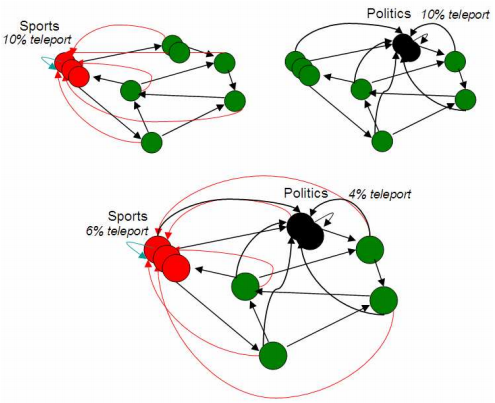
\includegraphics[width = 10cm]{Topic-specific_PageRank_Manning.png}
\item User have a mixture of interests - e.g. interest mixture 60\% and 40\% politics
\item Find a personalized PageRank for a user
\item Assume that an individual's interest can we well-approximated as a linear combination of a small number of topic page distributions
\item Leads to a Markov chain with a steady state distribution that is personalized
\item Implementation is cumbersome, demand that for each user need compute a transition matrix and steady-state distribution
\item Personalized PageRank vector can be expressed as a linear combination of underlying topic-specific PageRanks
\item E.g. Personalized PageRank $\vec{\pi} = 0.6\vec{\pi}_s + 0.4\vec{\pi}_p$ 
\end{itemize}
\section{Hubs and Authorities}
\begin{itemize}
\item Two primary kinds of web pages useful as results for broad-topic searches - informational query
\begin{itemize}
\item Authorities - pages with sources of information on a certain topic
\item Hubs - not in themselves sources of information, but compilations to authoritative pages
\end{itemize}
\item Circular definition - iterative computation
\end{itemize}
\section{Choosing the subset of the Web}
\begin{itemize}
\item Good authority pages may not contain the specific query term
\item Following procedure suggested: 
\begin{enumerate}
\item Given a query (e.g. leukaemia) use a text index to get all pages containing leukaemia, call this the \textit{root set} of pages
\item Build a \textit{base set} of pages, to include the root set as well as any page that either links to the a page in the root set, or is linked to by a page in the root set
\end{enumerate}
\item Then use the base set for computing hub and authority scores
\item Base set constructed in this way because:
\begin{enumerate}
\item A good authority page may not contain the query text
\item If the text query manages to capture a good hub page $v_h$ in the root set, then the inclusion of all pages inked to by any page in the root set will capture all the good authorities linked to by $v_h$ in the base set
\item Conversely, if the text query manages to capture a good authority page $v_a$ in the root set, then the inclusion of pages points to $v_a$ will bring other good hubs into the base set. In other words, the 'expansion' of the root set into the base set enriches the common pool of good hubs and authorities
\end{enumerate}
\item Suffices to use around 200 pages for the root set, rather than all pages matching the text query
\item A small number of iterations of the power method can compute a relative scoring of hubs and authorities
\item Shown around 5 iterations yield fairly good results
\end{itemize}
%--------------------------------------------------------------------
%--------------------------------------------------------------------
\end{document}